\documentclass[
%% TIKZ_CLASSOPTION %%
tikz
]{standalone}
\usepackage{amsmath}
\usetikzlibrary{matrix}
%% EXTRA_TIKZ_PREAMBLE_CODE %%
\begin{document}
%% TIKZ_CODE %%
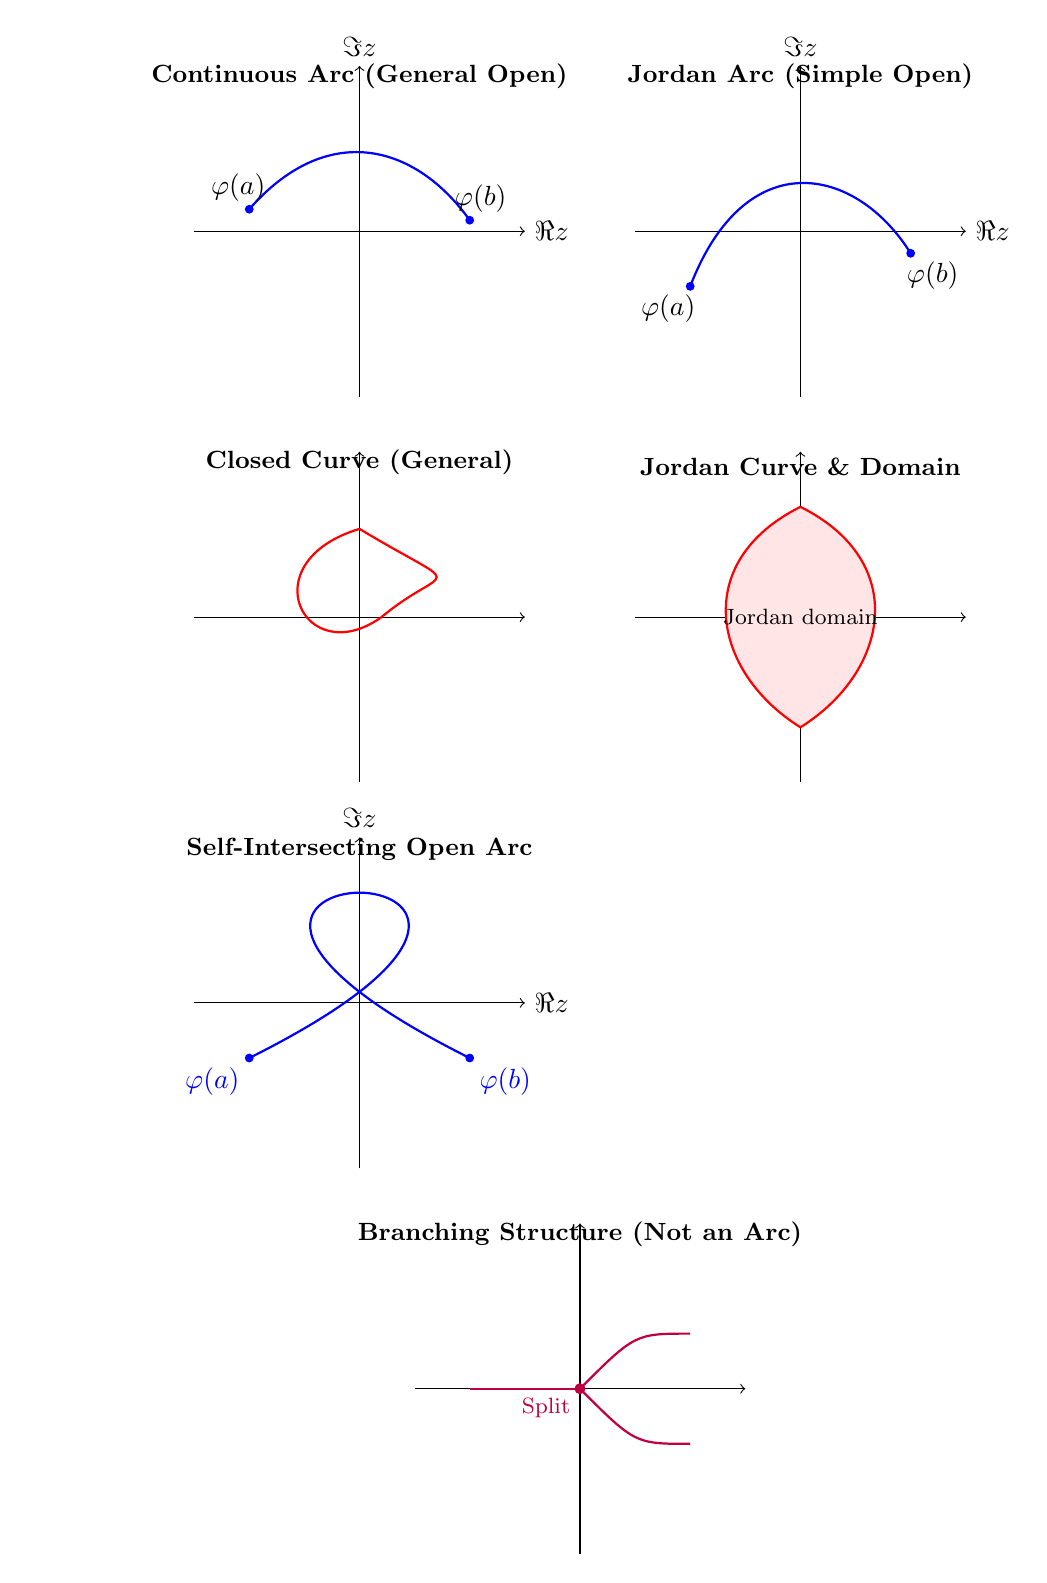
\begin{tikzpicture}[scale=1.4]

  % ====================================================
  % ROW 1: OPEN SIMPLE ARCS
  % ====================================================
  
  % TOP LEFT: Continuous Arc
  \begin{scope}[shift={(0,0)}]
    \node[above] at (0, 1.2) {\small \textbf{Continuous Arc (General Open)}};
    \draw[->] (-1.5,0) -- (1.5,0) node[right] {$\Re z$};
    \draw[->] (0,-1.5) -- (0,1.5) node[above] {$\Im z$};
    
    \draw[blue,thick] (-1,0.2) .. controls (-0.3,1.0) and (0.5,0.8) .. (1,0.1);
    \fill[blue] (-1,0.2) circle (0.04);
    \fill[blue] (1,0.1) circle (0.04);
    
    \node at (-1.1,0.4) {$\varphi(a)$};
    \node at (1.1,0.3) {$\varphi(b)$};
  \end{scope}

  % TOP RIGHT: Jordan Arc
  \begin{scope}[shift={(4,0)}]
    \node[above] at (0, 1.2) {\small \textbf{Jordan Arc (Simple Open)}};
    \draw[->] (-1.5,0) -- (1.5,0) node[right] {$\Re z$};
    \draw[->] (0,-1.5) -- (0,1.5) node[above] {$\Im z$};
    
    \draw[blue,thick] (-1,-0.5) .. controls (-0.5,0.8) and (0.5,0.6) .. (1,-0.2);
    \fill[blue] (-1,-0.5) circle (0.04);
    \fill[blue] (1,-0.2) circle (0.04);
    \node at (-1.2,-0.7) {$\varphi(a)$};
    \node at (1.2,-0.4) {$\varphi(b)$};
  \end{scope}

  % ====================================================
  % ROW 2: CLOSED STRUCTURES
  % ====================================================

  % MIDDLE LEFT: Closed Curve
  \begin{scope}[shift={(0,-3.5)}]
    \node[above] at (0, 1.2) {\small \textbf{Closed Curve (General)}};
    \draw[->] (-1.5,0) -- (1.5,0);
    \draw[->] (0,-1.5) -- (0,1.5);
    
    \draw[red,thick] 
      (0,0.8) .. controls (-1,0.5) and (-0.5,-0.5) .. 
      (0.2,0) .. controls (0.8,0.5) and (1,0.2) .. 
      (0,0.8);
  \end{scope}

  % MIDDLE RIGHT: Jordan Domain / Jordan Curve
  \begin{scope}[shift={(4,-3.5)}]
    \node[above] at (0, 1.2) {\small \textbf{Jordan Curve \& Domain}};
    \draw[->] (-1.5,0) -- (1.5,0);
    \draw[->] (0,-1.5) -- (0,1.5);
    
    \fill[red!10] 
      (0,1) .. controls (-1,0.5) and (-0.8,-0.5) .. 
      (0,-1) .. controls (0.8,-0.5) and (1,0.5) .. 
      (0,1);
      
    \draw[red,thick] 
      (0,1) .. controls (-1,0.5) and (-0.8,-0.5) .. 
      (0,-1) .. controls (0.8,-0.5) and (1,0.5) .. 
      (0,1);
      
    \node at (0,0) {\footnotesize $\text{Jordan domain}$};
  \end{scope}

% ====================================================
  % ROW 3: SELF-INTERSECTING NON-SIMPLE CASES
  % ====================================================

  % BOTTOM LEFT: Self-Intersecting Arc (FIXED COORDINATES)
  \begin{scope}[shift={(0,-7.0)}]
    \node[above] at (0, 1.2) {\small \textbf{Self-Intersecting Open Arc}};
    \draw[->] (-1.5,0) -- (1.5,0) node[right] {$\Re z$};
    \draw[->] (0,-1.5) -- (0,1.5) node[above] {$\Im z$};

    % Control points stretched out to (3, 1.5) and (-3, 1.5) to force the loop
    \draw[blue,thick]
      (-1,-0.5) .. controls (3,1.5) and (-3,1.5) .. (1,-0.5);

    \fill[blue] (-1,-0.5) circle (0.04) node[below left] {$\varphi(a)$};
    \fill[blue] (1,-0.5) circle (0.04) node[below right] {$\varphi(b)$};
  \end{scope}
  % ====================================================
  % ROW 4: NON-ARC STRUCTURE
  % ====================================================

  % CENTERED BOTTOM: Branching Structure
  \begin{scope}[shift={(2,-10.5)}]
    \node[above] at (0, 1.2) {\small \textbf{Branching Structure (Not an Arc)}};
    \draw[->] (-1.5,0) -- (1.5,0);
    \draw[->] (0,-1.5) -- (0,1.5);

    \draw[purple,thick] (-1,0) -- (0,0);
    \draw[purple,thick] (0,0) .. controls (0.5,0.5) .. (1,0.5);
    \draw[purple,thick] (0,0) .. controls (0.5,-0.5) .. (1,-0.5);

    \fill[purple] (0,0) circle (0.05) node[below left] {\footnotesize Split};
  \end{scope}
\end{tikzpicture} 
\end{document}
